\documentclass{article}
\usepackage{iclr2027_conference,times}
\usepackage[T1]{fontenc}
\usepackage[utf8]{inputenc}
\usepackage{amsmath,amssymb,mathtools}
\usepackage{graphicx,booktabs,multirow,tabularx,longtable,array}
\usepackage{float}
\usepackage{xcolor}
\usepackage{tikz}
\usepackage{algorithm,algorithmic}
\usepackage{hyperref,url}
\hypersetup{hidelinks,pdftitle={Learn the Task, Not the Schedule},pdfauthor={Anonymous}}
% All numerical result tables are placeholders until replaced by verified results.
\newcommand{\placeholdertable}[1]{{\color{red}\input{#1}}}
\newcommand{\method}{CTR}
\newcommand{\E}{\mathbb{E}}
\newcommand{\ind}{\mathbb{I}}
\newcommand{\R}{\mathbb{R}}
% Keep \iclrfinalcopy commented out for anonymous review.
%\iclrfinalcopy
\title{Learn the Task, Not the Schedule:\\Removing Demonstrator-Induced Scheduling\\Bias in Bimanual Imitation Learning}
\author{Anonymous authors}
\begin{document}
\maketitle
\vspace{-12pt}
\lhead{Under review as a conference paper at ICLR 2027}

\begin{abstract}
A bimanual demonstration specifies both \emph{what} the robot should do and one particular schedule for \emph{when} each arm should act.
Standard imitation learning does not distinguish task-required coordination from incidental scheduling choices, and may therefore learn to wait for the other arm or continue moving after its own work is done.
We study this failure mode as \emph{demonstrator-induced scheduling bias}: dependence on another arm's progress that is irrelevant for the current task phase.
We introduce Constraint-preserving Temporal Recombination (\method), a training-time data intervention that preserves recorded arm-local motion while pairing the same local behavior with multiple task-consistent relative schedules.
Task segments are annotated as reschedulable or protected by ordering/coordination constraints.
For recorded real-robot data, \method{} addresses two practical issues: reconstructing temporally consistent observations by compositing segmented arm-and-object foregrounds, and avoiding supervision during synthetic waits with an arm- and timestep-specific IdleMask.
Across Diffusion Policy, ACT, and $\pi_{0.5}$, we find that narrow demonstration schedules induce an almost one-for-one transfer of irrelevant other-arm delays: delaying one arm by 1\,s makes the irrelevant other-arm wait an extra $0.95$--$1.16$\,s, while \method{} reduces this to $0.21$\,s.
\method{} also reduces the success gap between seen and held-out joint-progress combinations from $6.8$ to $2.4$ percentage points.
Crucially, \method{} reduces sensitivity to irrelevant other-arm delays while preserving task-required coordination: in controlled real-robot prerequisite and shared-workspace tests, \method{} lowers constraint violations and more than halves the time to resume once the task can proceed.
Together, these results show that \method{} broadens the temporal contexts available during training, enabling bimanual policies to generalize across task-consistent schedules while preserving task-required coordination.

\end{abstract}

% Keep the teaser immediately below the complete abstract on the first page.
\begingroup
\setlength{\intextsep}{3pt}
\setlength{\abovecaptionskip}{4pt}
\begin{figure}[H]
\centering
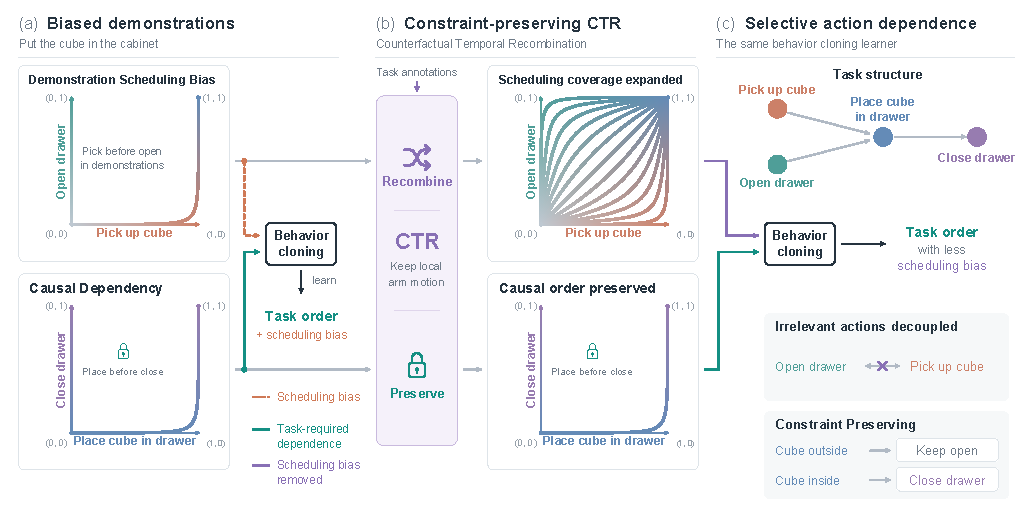
\includegraphics[width=.96\linewidth]{teaser/current/ctr_teaser_v4.pdf}
\caption{\method{} broadens admissible schedules while preserving local motion and task-required coordination, reducing demonstrator-induced scheduling bias.}
\label{fig:teaser}
\end{figure}
\endgroup

\section{Introduction}
A demonstration is simultaneously a skill trace and an answer to a scheduling question. Suppose one arm picks an object and the other arm picks a second, independent object. If the demonstrator happens to execute the two motions sequentially, the trajectory contains a useful manipulation strategy together with an incidental temporal convention. The same ambiguity appears inside coordinated tasks: opening a drawer must precede insertion, but it need not precede grasping the object that will eventually be inserted. A single demonstration realizes one feasible schedule; it does not say which temporal relationships define the task.

Modern visuomotor imitation policies, including Diffusion Policy (DP), Action Chunking with Transformers (ACT), and vision-language-action models, can fit expressive joint action distributions \citep{chi2023diffusion,zhao2023act,pi2025pi05}. But the demonstrations do not tell the policy whether a correlation between the two arms is required by the task or merely reflects the demonstrator's habit. When local progress is tightly correlated in training, the opposite arm becomes a reliable predictor of what to do next. The resulting policy may succeed under the nominal demonstration schedule while remaining brittle when one arm finishes early, pauses unexpectedly, or reaches a familiar local state alongside an unfamiliar other-arm state. We call this failure mode \emph{demonstrator-induced scheduling bias}.

The goal is not to make the arms independent, but to ignore incidental schedule correlations while preserving dependencies required by the task. During independent preparation, delaying one arm should not cause the other to wait. During insertion, support, alignment, or shared-workspace occupancy, the other arm's state may be exactly the information the policy must respond to.

We address this question with \method{} (Figure~\ref{fig:teaser}). \method{} keeps the recorded local sensorimotor content of each arm fixed while varying only its admissible timing relative to the other arm. We use GPT-6 Astra to construct task-level temporal annotations and generate task-specific video-annotation programs. On recorded real-robot data, we reconstruct the corresponding main-view observations from recognized and segmented arm/object foregrounds, and use IdleMask so that artificially inserted waits are not learned as expert actions. The policy architecture and inference procedure are unchanged; no task graph or scheduler is queried at deployment.

Our contribution is organized around the failure mode rather than benchmark success alone. First, we formulate schedule dependence as a behavioral invariance problem and make explicit what is and is not identifiable from demonstrations. Second, we introduce \method{} as a constraint-preserving intervention on the training timing distribution, including a real-robot data realization and a principled treatment of synthetic waiting labels. Third, we establish a controlled behavioral evaluation protocol for schedule inheritance, robustness, selective coordination, and joint-progress generalization across DP, ACT, and $\pi_{0.5}$.

\section{Related work}
\paragraph{Causal confusion and counterfactual augmentation.}
Imitation learners can exploit predictive but non-causal features of expert data \citep{dehaan2019causal}. CoDA recombines locally factored transition components \citep{pitis2020coda}, CAIAC exchanges state components estimated to be unaffected by an action \citep{urpi2024caiac}, and RoCoDA applies counterfactual state recombination to visual robot imitation, including bimanual manipulation \citep{ameperosa2025rocoda}. We study a structured nuisance variable that is especially visible in bimanual data: relative execution progress. Our focus is the behavioral failure induced by narrow schedule coverage and how to evaluate it with controlled execution interventions.

\paragraph{Demonstration generation and multi-arm retiming.}
MimicGen adapts object-centric demonstration segments to new contexts \citep{mandlekar2023mimicgen}; DexMimicGen extends automated generation to bimanual dexterous manipulation with asynchronous execution and synchronization constraints \citep{jiang2025dexmimicgen}. TriManPolicy retimes multi-arm sensorimotor segments under dependency and resource constraints \citep{zhao2026triman}. \method{} uses retiming for a different objective: expose the same local behavior to multiple legal other-arm progress contexts so that a joint imitation policy cannot rely on one narrow demonstration schedule. Our evaluation therefore centers on paired other-arm pause interventions and held-out joint-progress combinations rather than makespan alone.

\paragraph{Architectural separation and skill composition.}
The Decoupled Interaction Framework separates arm policies while allowing selective interaction \citep{jiang2025dif}, and SkillVLA studies reuse across novel left--right skill pairings \citep{zhai2026skillvla}. These approaches change model structure or skill composition. \method{} changes the training distribution while retaining the chosen joint policy architecture, allowing the same failure mode and training-time intervention to be tested across DP, ACT, and $\pi_{0.5}$.

\section{Problem formulation: task dependence versus schedule dependence}
\subsection{A behavioral failure mode}
Let a demonstration contain observations $o_t=(I_t^{\rm main},I_t^L,I_t^R,q_t^L,q_t^R)$ and actions $a_t=(a_t^L,a_t^R)$. Let $p_i$ denote arm $i$'s local semantic progress, $x_i$ its task-relevant local state, $c$ the shared conditions that determine whether cross-arm coordination is required, and $z_{\bar i}$ the remaining aspects of the opposite arm's progress.

During a phase in which $z_{\bar i}$ is irrelevant, correct behavior should be approximately invariant to admissible changes in that other-arm context:
\begin{equation}
 \pi_i(\cdot\mid x_i,c,z_{\bar i})
 \approx
 \pi_i(\cdot\mid x_i,c,z'_{\bar i}).
 \label{eq:invariance}
\end{equation}
A policy exhibits scheduling bias when changing only the admissible progress of the other arm produces a systematic change in its own otherwise feasible behavior. This definition is deliberately phase-specific. If the other arm withholds a prerequisite, removes support, breaks alignment, or occupies a required workspace, then $c$ changes and invariance is no longer the desired behavior.

\subsection{What is and is not identifiable}
If every observed demonstration satisfies $A\prec B$, the same data are compatible with two different explanations: $A$ may be a genuine prerequisite for $B$, or the demonstrator may simply prefer a serial scheduler. The left/right action partition identifies where a controlled pause can be applied, but it does not resolve this ambiguity. Objects, contacts, visibility, support, and shared geometry can create real dependencies between arms.

\method{} therefore does not attempt to discover the complete task constraint graph from demonstrations alone. Instead, \method{} uses training-time annotations of task temporal constraints. These annotations are supervision for data construction; they are not policy inputs and are not queried at deployment.

The target is \emph{behavioral selectivity}: reduce sensitivity to progress of the other arm when the annotated task relation says that progress is irrelevant, while retaining sensitivity when the other arm changes a binding task condition. \method{} is a training-time data intervention in this sense: it alters the timing distribution used for learning, while claims concern observable policy behavior rather than recovery of a hidden neural causal graph.

\section{Constraint-Preserving Temporal Recombination}
Figure~\ref{fig:method} summarizes the data-processing pipeline.
Our goal is to isolate the effect of demonstration timing. Recollecting demonstrations under different schedules would also change the executed trajectories, introducing additional confounds. CTR instead preserves the recorded arm-local behavior and varies only admissible relative timing, making schedule the primary manipulated factor. The same property also makes CTR a practical data-augmentation method: it expands schedule coverage from existing demonstrations without requiring additional robot data collection.
\subsection{Annotate rescheduling degrees of freedom}
We decompose each recorded demonstration into ordered arm-local segments. GPT-6 Astra identifies the temporal dependency relations for the task, including which segment relations are reschedulable and which must be protected. Its generated video-annotation program then annotates the temporal segments in the recorded demonstrations. Intervals that may be shifted relative to the opposite arm are reschedulable, while within-arm ordering and task-required cross-arm relations are protected. The protected set includes prerequisites, sustained support, cooperative alignment, and shared-workspace exclusion. Coupled blocks move together; independent blocks may become serial, overlapping, or partially overlapping.

A schedule $s$ specifies segment start times, and $\Omega(\tau)$ denotes the admissible schedules for demonstration $\tau$. The annotation layer defines $\Omega(\tau)$; the policy never sees these labels. This separation is central to the study: task knowledge is used to construct alternative supervision, then distilled into an ordinary joint imitation policy.

\subsection{Recombine time while preserving local motion}
For arm $i$, a source-time map $\phi_i^s(t)$ selects the recorded state and action corresponding to its local progress under schedule $s$. Inside an active segment, sample order and local motion are unchanged. Only the relative timing between compatible arm-local streams is varied. Training examples are drawn from
\begin{equation}
 \widetilde{\mathcal D}
 =\left\{\mathcal C\bigl(\tau,\phi_L^s,\phi_R^s\bigr):
 \tau\in\mathcal D,
 s\sim q(\cdot\mid\Omega(\tau))\right\},
 \label{eq:dataset}
\end{equation}
where $\mathcal C$ aligns the selected observation and action streams and $q$ samples multiple admissible relative schedules. Rather than choosing a small set of discrete schedules, \method{} samples relative timing uniformly across the admissible range, exposing the same local arm behavior to many legal states of opposite-arm progress.

\begin{figure}[t]
\centering
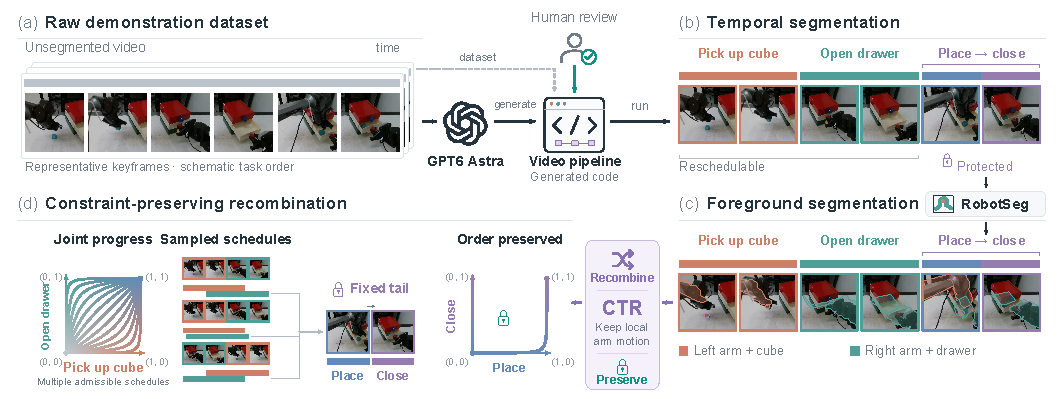
\includegraphics[width=\linewidth]{ctr_pipeline/ctr_pipeline.pdf}
\caption{\method{} data-processing pipeline. Foreground segmentation supports observation composition, and temporal recombination varies compatible arm-local schedules while preserving local motion and protected ordering. The displayed masks and sampled schedules are schematic.}
\label{fig:method}
\end{figure}

\subsection{CTR on recorded real-robot data: two implementation issues}
CTR has two implementation issues in recorded real data:
\begin{enumerate}
    \item reconstruct temporally consistent observations;
    \item avoid treating synthetic waits as expert decisions.
\end{enumerate}
These are consequences of the same intervention: changing relative arm progress changes what the cameras should show and can create timeline gaps that were never expert actions.

\paragraph{Issue 1: reconstruct observations by visual composition.}
Each wrist view and proprioceptive stream is selected at its own arm's source time. For the main camera, RobotSeg and related open-source recognition/foreground-segmentation tools identify the two arms and task-relevant objects and extract foreground masks. Let $F_i$ and $M_i$ denote the selected foreground and mask for arm $i$, and let $B$ denote the scene background. We compose
\begin{equation}
 \widetilde I_t^{\rm main}
 =\operatorname{Compose}\!\left(
 B,
 M_L(\phi_L^s(t))\odot F_L(\phi_L^s(t)),
 M_R(\phi_R^s(t))\odot F_R(\phi_R^s(t))\right).
 \label{eq:compose}
\end{equation}
The resulting main-view sequence approximates the appearance of both arms executing the recombined schedule concurrently, without requiring a simulator or digital twin. Because protected contact and coupled stages are not independently retimed, visual composition is used only for temporal combinations admitted by the task annotations.

\paragraph{Issue 2: remove synthetic waiting from supervision.}
A sampled schedule may insert a delay between valid local segments. That delay is useful for constructing the joint temporal context, but it does not mean an expert chose to wait in the resulting visible state. For batch element $b$, prediction step $k$, arm $i$, and action coordinate $d$, define $m_{bkid}=0$ on artificially inserted waiting coordinates and $m_{bkid}=1$ otherwise. The base imitation loss becomes
\begin{equation}
 \mathcal L_{\rm action}
 =\frac{\sum_{b,k,i,d}m_{bkid}\,\ell_{bkid}}
        {\max(1,\sum_{b,k,i,d}m_{bkid})}.
 \label{eq:loss}
\end{equation}
Here $\ell$ is the coordinatewise action, denoising, or velocity-prediction loss of the underlying learner. IdleMask removes only artificial waiting targets. Required holding, active support, and terminal holding remain supervised. \method{} introduces no deployment-time scheduler and no additional pairwise consistency loss.

\section{Experimental design: five questions about scheduling bias}
Our evaluation asks five questions that separate the existence of demonstrator-induced scheduling bias from its consequences and from the desired selectivity of the solution. \textbf{Q1:} Does changing the demonstration schedule change the execution schedule learned by the policy? \textbf{Q2:} Does narrow schedule coverage make cross-arm behavior brittle even when local skills are unchanged? \textbf{Q3:} Does delaying an irrelevant other arm cause the unfrozen arm to wait? \textbf{Q4:} Can we reduce unnecessary cross-arm dependence without weakening task-required coordination? \textbf{Q5:} Does broader schedule coverage improve generalization to unseen combinations of familiar local progress? A final component study isolates the roles of temporal variation, IdleMask, and the reconstructed main view.

\paragraph{Controlled timing distributions.}
The mechanism study uses the same local segment content to construct five training distributions: \textbf{Original}, the recorded demonstrations as collected; \textbf{Sequential}, which reverses the relative execution order in Original (e.g., $L\!\rightarrow\!R$ becomes $R\!\rightarrow\!L$); \textbf{Concurrent}, which aligns the two arms to start at the same time; \textbf{Mixed}, which mixes Sequential and Concurrent demonstrations; and \textbf{\method}, which uniformly samples relative schedules across the full admissible range from fully left-before-right to fully right-before-left. Intermediate \method{} samples include partially overlapping and approximately concurrent executions. These transformations are applied only to task segments annotated as reschedulable; protected prerequisites, cooperative interactions, support/alignment relations, and workspace constraints remain unchanged. Thus, the left-before-right and right-before-left endpoints refer to the admissible ordering of reschedulable task segments, not to reordering an entire task when protected cross-arm dependencies are present. Training data volume and update count are matched within each model.

\paragraph{Tasks and models.}
We evaluate four classes of bimanual tasks: (i) \emph{independent} tasks, where the two arms' subtasks are unrelated; (ii) \emph{dependency} tasks, where one arm's progress is a prerequisite for the other; (iii) \emph{coordinated} tasks, where the two arms must act in tight coordination; and (iv) \emph{workspace-exclusion} tasks, where the arms cannot occupy the relevant workspace simultaneously. For each class, we select one simulated and one real-robot task from RoboTwin2, yielding four simulated and four real tasks in total (Appendix~\ref{app:tasks}). We evaluate DP, ACT, and $\pi_{0.5}$ in the controlled timing, paired-pause, held-out-progress, and eight-task coordination studies, and DP/$\pi_{0.5}$ in the component study.

\paragraph{Diagnostics.}
For the schedule-reversal test, we measure the relative start time
\begin{equation}
 \Delta_{\rm start}=t_R^{\rm start}-t_L^{\rm start},
 \label{eq:start-order}
\end{equation}
where positive values indicate left-first execution, negative values indicate right-first execution, and values near zero indicate approximately simultaneous starts. We also report task success (SR), capped completion time $T_{\rm cap}$, unnecessary ready-state waiting $W_i$, and post-completion end-effector translation $M_i$. Paired-pause effects $\Delta W_i$ measure extra waiting in the \emph{unfrozen} arm. Constraint tests report dependency violations (DVR), exclusion violations (XR), release latency, and nonresponse after a prerequisite or shared region becomes available. Operational definitions and the full condition-level tables are in the appendix. Main-text averages are descriptive macro-averages over the stated cells.

\section{Diagnosing demonstrator-induced scheduling bias}
\subsection{Changing the demonstration schedule changes the learned execution schedule}
We first test whether scheduling bias in the demonstrations appears directly in the learned policy. PutCub contains two independent subtasks, so either arm may start first without changing the task. We compare \textbf{Original} with \textbf{Sequential}, which preserves the local task content but reverses the relative execution order of the two arms. Both policies are evaluated from the same C0 initial condition. Because the local behaviors are held fixed, a systematic change in $\Delta_{\rm start}$ isolates sensitivity to the demonstration schedule itself. If the policy learned only task-required structure, reversing an incidental demonstration order should not systematically reverse its execution order; if it inherits the demonstrator's scheduling bias, the sign of $\Delta_{\rm start}$ should reverse between Original and Sequential.

% TODO(author): The current repository export does not contain Delta_start or an equivalent
% execution-order statistic. Insert the scheduler-reversal result here once the metric/table
% has been exported. Do not reuse illustrative numbers from earlier drafts unless they are
% verified against the final experiment logs.

\subsection{Narrow schedule coverage creates brittle cross-arm behavior}
PutCub is evaluated from three initial conditions: both subtasks unfinished (C0), left already complete (CL), and right already complete (CR). CL and CR change the other arm's progress without changing the unfinished arm's remaining task. Table~\ref{tab:e1} shows a consistent pattern across all three policy families.

\begin{table}[t]
\caption{Completion-state stress test on PutCub under five training timing distributions. $W_{\rm unfinished}$ (s) measures unnecessary waiting of the arm that still has work to do; $M_{\rm complete}$ (cm) measures motion of the arm whose responsibility is already complete.}
\label{tab:e1}
\centering\small\setlength{\tabcolsep}{3pt}
\placeholdertable{tables/e1_main.tex}
\end{table}

All three single-schedule groups degrade when one arm is already finished: averaged over models and CL/CR, success is 59.9\%, 61.2\%, and 60.7\% for Original, Sequential, and Concurrent. Mixed raises this to 70.1\%, confirming that schedule diversity itself matters. \method{} reaches 79.1\%. Relative to Mixed, unfinished-arm waiting falls from 2.56\,s to 1.21\,s, while completed-arm translation falls from 2.71\,cm to 1.31\,cm.

The failure is not specific to one execution order: Original, Sequential, and Concurrent are all brittle to changes in the other arm's progress, and Mixed only partly fixes this. This shows that inheriting a narrow schedule is not merely a harmless preference; it makes the policy brittle when familiar local behavior is paired with different other-arm progress.

\subsection{Pausing an irrelevant arm transfers waiting to the other arm}
In independent PutCub phases, we compare a normal execution with a matched branch in which only one arm is forced to remain still for 1, 2, or 4 seconds. The other arm continues to receive observations and control normally. For the unfrozen arm $i$,
\begin{equation}
 \Delta W_i(d)=\frac{1}{P}\sum_{j=1}^P
 \left(W_{ij}^{\operatorname{pause}(\bar i,d)}-W_{ij}^{\rm control}\right).
 \label{eq:paired_pause}
\end{equation}
If the current task phase is independent, a policy that learned the task rather than the demonstration schedule should have a small transferred-delay response.

\begin{figure}[t]
\centering
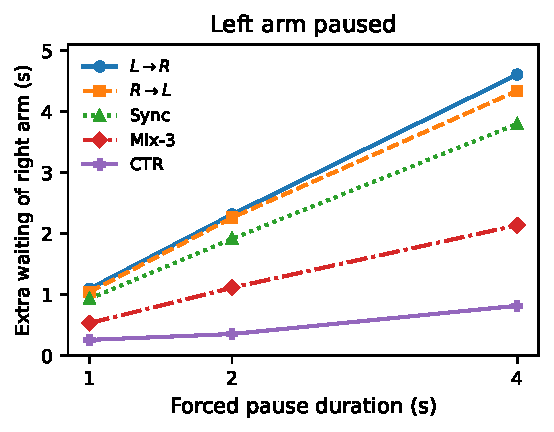
\includegraphics[width=.49\linewidth]{figures/freeze_L.pdf}\hfill
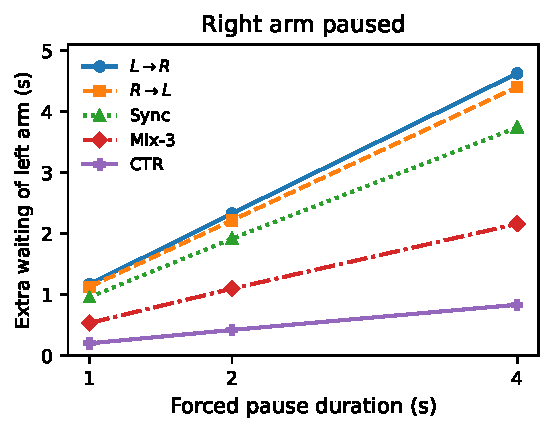
\includegraphics[width=.49\linewidth]{figures/freeze_R.pdf}
\caption{Paired other-arm pause intervention. Pausing one otherwise irrelevant arm induces unnecessary waiting in the unfrozen arm. Each point averages DP, ACT, and $\pi_{0.5}$ for one pause direction and duration; all condition-level results appear in Appendix~\ref{app:e2a}.}
\label{fig:freeze}
\end{figure}

Extra waiting grows with pause duration. At a four-second pause, macro-averaged extra waiting is 4.62\,s for Original, 4.38\,s for Sequential, 3.77\,s for Concurrent, and 2.15\,s for Mixed, but only 0.83\,s for \method---a 61.5\% reduction relative to Mixed. Joint success under the same pauses averages 68.9\% for Mixed and 78.4\% for \method, ruling out the trivial explanation that a low $\Delta W$ comes from a policy that simply stops acting.

The same diagnostic appears in the real-robot component cohort. Across block sorting (R1) and screw--sleeve insertion (R3), DP and $\pi_{0.5}$ average 2.86\,s extra waiting for Fixed, 1.85\,s for Fixed+Mask, and 0.48\,s for \method. The paired pause intervention therefore measures the failure mode directly: narrow demonstration schedules make the other arm's progress behaviorally predictive even when the task phase does not require that dependence.

\section{Removing schedule bias without removing coordination}
A policy could trivially reduce other-arm sensitivity by ignoring the other arm. That would fail exactly where coordination is necessary. We therefore evaluate \method{} on eight tasks covering independent work, prerequisites, alignment, and shared-workspace exclusion, and then test the binding conditions themselves.

\begin{table}[t]
\caption{Default-condition success (\%) on four simulated and four real tasks. Each pair compares original demonstrations with \method{} using the same policy family.}
\label{tab:generality}
\centering\small\setlength{\tabcolsep}{5pt}
\placeholdertable{tables/e3_main.tex}
\end{table}

Across all 24 task--model comparisons in Table~\ref{tab:generality}, \method{} has higher reported success. The macro-average rises from 68.3\% to 85.4\% in simulation and from 62.7\% to 79.5\% on real hardware. More importantly for the failure-mode claim, gains do not come from indiscriminate parallelization.

For prerequisite tasks we delay and then release the binding condition; for shared-workspace tasks we occupy and then release the conflict region. A correct policy should wait while the constraint is active and resume promptly when it disappears. Table~\ref{tab:constraints} reports both the violation rate and the release response.

\begin{table}[t]
\caption{Selective-coordination interventions, averaged over models within each task. Violation is DVR for prerequisite/alignment tasks and XR for shared-workspace tasks. Release measures latency after the prerequisite or workspace becomes available.}
\label{tab:constraints}
\centering\small\setlength{\tabcolsep}{5pt}
\placeholdertable{tables/constraints_main.tex}
\end{table}

On the real drawer task, prerequisite violations fall from 6.30\% to 1.75\% and release latency from 1.56\,s to 0.64\,s. On real shared-workspace sorting, exclusion violations fall from 4.99\% to 2.31\% and release latency from 1.57\,s to 0.69\,s. On screw--sleeve insertion, where execution moves from independent preparation to cooperative insertion and back to independent completion, the independent-after-cooperation condition improves from 57.3\% to 74.0\% success. Across the four real default tasks, collision rates decrease from 3.20\% to 1.50\% and safety-intervention rates from 3.89\% to 1.75\%.

Together with the paired-pause diagnostic, these tests show the selective pattern we seek: less transferred waiting when progress of the other arm is irrelevant, but stronger respect for prerequisites, alignment, and workspace constraints when the other arm's state is task-binding.

\section{Generalization to held-out joint-progress combinations}
The previous experiments establish the failure and test whether \method{} removes the wrong dependence without removing required coordination. We next ask whether broader schedule coverage also improves compositional generalization. We train separate models after withholding designated regions of joint semantic progress. H1 contains $p_L\in[0.4,0.6]$ with $p_R\in[0,0.1]$; H2 mirrors this split; H3 is the supplied late-mid/early-mid holdout. Each arm's local progress states are represented elsewhere in training, while the selected pairings are not.

\begin{table}[t]
\caption{Performance on seen and held-out joint-progress combinations, macro-averaged over three models and three holdout splits. Gap is seen SR minus held-out SR in percentage points; waiting is summed over arms (s).}
\label{tab:heldout}
\centering\small\setlength{\tabcolsep}{4pt}
\placeholdertable{tables/e2b_main.tex}
\end{table}

Table~\ref{tab:heldout} shows the separation between discrete schedule mixing and broader joint-progress coverage. Mixed reaches 69.9\% held-out success with a 6.8-point seen-to-held-out gap. \method{} reaches 79.8\% held-out success and reduces the gap to 2.4 points. Held-out total waiting falls from 4.30\,s to 1.99\,s. The local behaviors are not new; what is new is their pairing. This directly tests whether broader temporal coverage helps the policy combine familiar local behaviors in unseen joint contexts.

\section{What makes CTR work?}
The component study separates the data intervention from its two real-data implementation components. We evaluate Fixed, Fixed+Mask, \method{} without IdleMask, full \method, \method{} without the main view, and a directly collected multi-schedule reference (Real-Multi). Table~\ref{tab:ablation} averages real R1/R3 conditions for DP and $\pi_{0.5}$.

\begin{table}[t]
\caption{Real-robot component study on R1/R3 with DP and $\pi_{0.5}$. Labels is the reported number of valid supervised action elements in millions; $W$ is waiting (s), $M$ post-completion motion (cm), and $\Delta W$ paired extra waiting (s).}
\label{tab:ablation}
\centering\small\setlength{\tabcolsep}{4pt}
\placeholdertable{tables/e4_main.tex}
\end{table}

\paragraph{Temporal variation does more than mask waiting labels.}
Fixed+Mask lowers waiting relative to Fixed, but full \method{} is substantially stronger under the matched reported count of 0.93 million valid action elements: success increases from 68.2\% to 75.6\%, total waiting falls from 3.41\,s to 1.17\,s, and paired extra waiting falls from 1.85\,s to 0.48\,s. The policy benefits from seeing the same local behavior under different legal other-arm progress contexts, not only from deleting idle targets.

\paragraph{IdleMask matters once schedules are recombined.}
Without IdleMask, temporal recombination still improves over Fixed, but success is 71.9\% rather than 75.6\% and extra waiting is 1.32\,s rather than 0.48\,s. Synthetic waits are therefore not neutral labels: supervising them partly reinstates the scheduling behavior that \method{} is designed to remove.

\paragraph{The reconstructed main view carries useful cross-arm context.}
Removing the main view lowers average success from 75.6\% to 71.5\% and raises extra waiting from 0.48\,s to 1.00\,s. Real-Multi reaches 74.3\% success and 0.67\,s extra waiting, providing a useful reference for what broad schedule coverage can achieve when it is collected directly rather than synthesized. Detailed per-task results and label-count differences are reported in Appendix~\ref{app:e4}.

\section{Limitations}
\method{} depends on correct training-time temporal annotations; annotation errors can create invalid recombinations. Main-view composition is also an approximation to a physically realized concurrent scene, which is why contact-sensitive and coupled segments remain protected rather than being independently recombined. Finally, the paired other-arm pauses and held-out progress regions cover specific forms of other-arm dependence rather than every possible bimanual interaction. These limitations narrow the claim to demonstrator-induced scheduling bias under annotated task constraints, while leaving the intervention and diagnostics directly testable.

\section{Conclusion}
Imitation policies can inherit incidental scheduling conventions from bimanual demonstrations. \method{} reduces this bias by exposing the same local behaviors to diverse task-consistent schedules while preserving required coordination. Across schedule reversal, other-arm interventions, coordination tests, and held-out joint contexts, the results support the same goal: learned cross-arm dependence should reflect the task, not the demonstrator's schedule.
\label{sec:mainend}

\clearpage
\section*{Reproducibility statement}
The source package contains the condition-level aggregate exports, CSV conversions, scripts that regenerate the descriptive tables and paired-pause plots, and the LaTeX source. Appendix~\ref{app:metrics} gives the metric definitions and Appendix~\ref{app:implementation} specifies the \method{} data-construction pipeline. A complete experimental release should include GPT-6 Astra temporal-relation annotations, the generated video-annotation programs, and prompt/schema versions, as well as the RobotSeg and foreground-processing configuration, source-to-recombined trajectory links, schedule samples, masks, policy configurations, and episode-level evaluation logs.

\section*{Ethics statement}
Temporal recombination is applied only within task-annotated admissible regions; prerequisites, sustained support, shared-object interactions, and workspace exclusions remain protected. Real-robot deployment uses the same independent safety procedures as the baseline policies. Any release of recorded camera streams should respect consent, privacy, and applicable data-use permissions.

\section*{AI use statement}
GPT-6 Astra has two roles in the data-construction pipeline: identifying the temporal dependency relations for each task, including which are reschedulable and which must be protected, and generating the automatic video-annotation programs that label temporal segments in recorded demonstrations. Generative AI was also used to discuss hypotheses and experimental design, assist literature discovery and comparison, formalize the method, analyze aggregate results, and draft and edit the manuscript and LaTeX. The robot experiments and reported empirical outcomes are produced by the experimental pipeline rather than by the writing model.

\bibliographystyle{plainnat}
\bibliography{references}
\clearpage
\appendix
\section{Task and evaluation inventory}
\label{app:tasks}
Table~\ref{tab:tasks} maps the task identifiers used throughout the paper to their dependency structure. PutCub is the separate two-subtask cabinet task used for the mechanism, paired-pause, and held-out joint-progress studies.

\begin{table}[ht]
\caption{Task mapping and protected temporal relationships. ``Independent'' refers to the indicated task phase; protected interactions remain unchanged during recombination.}
\label{tab:tasks}
\centering\small
\begin{tabularx}{\linewidth}{llXX}
\toprule
ID & Domain & Task & Temporal structure used by CTR \\
\midrule
PutCub & Sim. & Put Object in Cabinet; two independent subtasks & Preserve each local sequence; relative progress may vary across the two subtasks.\\
S1 & Sim. & Each arm acquires a bottle & Separate objects and independent progress.\\
R1 & Real & Each arm sorts its own blocks & Separate sorting subtasks and terminal holds.\\
S2 & Sim. & Place an object in a drawer & Opening precedes insertion; independent object preparation may overlap.\\
R2 & Real & Place a block in a drawer & Same prerequisite and holding structure.\\
S3 & Sim. & Scan Object & Independent preparation followed by protected relative pose/alignment during scanning.\\
R3 & Real & Insert a screw into a sleeve & Independent acquisition, protected cooperative insertion, independent completion.\\
S4 & Sim. & Place two shoes in a shared receptacle & Independent preparation with protected shared-workspace exclusion.\\
R4 & Real & Sort mixed workpieces into left/right boxes & Protected shared-space exclusion and affected-object state.\\
\bottomrule
\end{tabularx}
\end{table}

\paragraph{Evaluation inventory.}
All result cells use three training seeds. Experiment~1 contains three models, five training timing distributions, and three initial conditions, with 180 evaluations per cell. The paired-pause study contains three models, five timing distributions, two pause directions, and 1/2/4-second durations; each condition contains 60 matched pairs (120 branch executions). The held-out joint-progress study uses 90 seen and 90 held-out evaluations per cell. The eight-task generality study uses 150 evaluations per simulated cell and 60 per real-robot cell. The component study uses DP and $\pi_{0.5}$ on PutCub, R1, and R3, with its full condition-level results reported in Appendix~\ref{app:e4}.

\paragraph{Training groups.}
Mix-3 is a single training set containing equal contributions from left-first, right-first, and simultaneous-start schedules; it is not an ensemble. The local arm content and training/update budgets are matched within the controlled timing experiment. Completed-arm holding examples are retained whenever holding is part of the task semantics.

\section{Metric definitions and aggregation}
\label{app:metrics}

\subsection{Success and failure-penalized completion time}
For evaluation $j$, let $T_j$ be the task-specific time limit, $S_j\in\{0,1\}$ indicate task success, and $t_j^{\rm goal}$ be completion time when successful. We report
\begin{equation}
 \mathrm{SR}=100\frac{1}{N}\sum_{j=1}^{N} S_j,
 \qquad
 T_{\rm cap}=\frac{1}{N}\sum_{j=1}^{N}
 \left[S_jt_j^{\rm goal}+(1-S_j)T_j\right].
 \label{eq:metrics-success}
\end{equation}
Failures and safety aborts therefore remain in the time metric through the task limit.

\subsection{Unnecessary waiting}
Let $r_{ij}(t)=1$ when arm $i$ still has an unfinished responsibility and can make legitimate task progress: required prerequisites are satisfied and there is no required hold or true obstruction. Let $b_{ij}(t)=1$ when the arm remains below the motion/progress thresholds used by the evaluator. If $\mathcal J_{ij}$ is the set of maximal intervals satisfying $r_{ij}(t)b_{ij}(t)=1$ for longer than the idle threshold, then
\begin{equation}
 W_{ij}=\sum_{J\in\mathcal J_{ij}} |J|,
 \qquad
 W_i=\frac{1}{N}\sum_j W_{ij}.
 \label{eq:metrics-wait}
\end{equation}
Necessary support or prerequisite waiting does not count as unnecessary waiting. When a total is reported, $W=W_L+W_R$.

In Experiment~1, unfinished-arm waiting is $W_R$ in CL and $W_L$ in CR. The main-table summary averages these two values.

\subsection{Post-completion motion}
Let $c_{ij}$ be the end of all responsibilities of arm $i$, including any required support or retreat, and let $x_{ij,k}\in\R^3$ be its end-effector position. Over a post-completion observation window $\tau_{\rm post}$,
\begin{equation}
 M_{ij}=100\sum_{k:\,[t_k,t_{k+1}]\subset[c_{ij},c_{ij}+\tau_{\rm post}]}
 \|x_{ij,k+1}-x_{ij,k}\|_2,
 \label{eq:metrics-motion}
\end{equation}
where the factor 100 converts meters to centimeters. In CL/CR summaries, $M_L$ is used for CL and $M_R$ for CR.

\subsection{Paired other-arm pause effects}
For pair $j$, we execute a control branch and a matched branch that pauses only the opposite arm $\bar i$ for duration $d$. For the unfrozen arm $i$,
\begin{equation}
 \delta W_{ij}=W_{ij}^{\rm pause}-W_{ij}^{\rm control},
 \qquad
 \Delta W_i=\frac{1}{P}\sum_j\delta W_{ij}.
 \label{eq:metrics-paired}
\end{equation}
The analogous $\Delta T_{{\rm cap},i}$ measures the change in failure-penalized time for the unfrozen arm's remaining responsibility.

\subsection{Constraint, collision, and safety events}
Let $D_j$ indicate an attempted action before a required prerequisite or an invalid withdrawal of required support; $X_j$ a forbidden concurrent workspace occupancy; $C_j$ a disallowed collision; and $A_j$ a safety-controller intervention or abort. We report
\begin{equation}
 (\mathrm{DVR},\mathrm{XR},\mathrm{CR},\mathrm{SAR})
 =\frac{100}{N}\sum_j(D_j,X_j,C_j,A_j).
 \label{eq:metrics-constraint}
\end{equation}
DVR and XR are task-specific metrics rather than a single pooled notion of violation.

\subsection{Responding after a binding condition is released}
For a valid release event $e$, let $t_e^{\rm ready}$ be the first time that a previously withheld prerequisite or occupied region becomes available, $t_e^{\rm act}$ the first appropriate task-progress action, and $H_e$ the response horizon. We use
\begin{equation}
 L_e=\min(t_e^{\rm act}-t_e^{\rm ready},H_e),\qquad
 U_e=\ind[t_e^{\rm act}-t_e^{\rm ready}>H_e],
 \label{eq:metrics-release}
\end{equation}
with $L_e=H_e$ and $U_e=1$ if no response occurs. Release latency and nonresponse complement the violation metric: a policy should both respect an active constraint and resume when the constraint disappears.

\subsection{Aggregation}
Main-text macro-averages are unweighted means over the explicitly named task/model/condition cells, computed before display rounding. Detailed tables retain the condition-level interval fields from the experiment export. We do not pool heterogeneous tasks into a raw-time average when their evaluation horizons differ.

\section{CTR implementation details}
\label{app:implementation}

\begin{algorithm}[ht]
\caption{CTR data-construction algorithm}
\label{alg:ctr}
\begin{algorithmic}[1]
\REQUIRE Recorded streams $\mathcal D$; task description; training budget
\FOR{each selected recorded demonstration $\tau$}
\STATE Segment the trajectory into ordered arm-local task intervals.
\STATE Use GPT-6 Astra to identify the task's temporal dependency relations, marking each as reschedulable or protected.
\STATE Run the video-annotation program generated by GPT-6 Astra to label temporal segments in the recorded demonstration.
\STATE Build $\Omega(\tau)$ by preserving within-arm order, prerequisites, cooperative/support blocks, alignment, and workspace exclusion.
\STATE Sample an admissible relative schedule $s\in\Omega(\tau)$.
\FOR{each selected output time $t$}
\STATE Read each arm's wrist view, proprioception, and valid local action at source time $\phi_i^s(t)$.
\STATE For real data, use RobotSeg-style recognition/segmentation to extract the selected arm/object foregrounds and compose the main view.
\STATE Set IdleMask to zero only for waiting coordinates inserted by the sampled schedule.
\STATE Retain supervision for valid motion, required support, and terminal holding.
\ENDFOR
\ENDFOR
\STATE Train the chosen joint policy with the masked base imitation objective and matched update budget.
\STATE Deploy on ordinary real observations; no temporal annotations or scheduler are queried online.
\end{algorithmic}
\end{algorithm}

\subsection{GPT-6 Astra roles}
GPT-6 Astra has two roles in CTR. First, it identifies the temporal dependency relations for each task, including which relations are reschedulable and which must be protected. Protected relations are further represented as precedence, cooperative/synchronized execution, sustained support, alignment-sensitive interaction, or shared-workspace exclusion when needed by the task. Second, it generates an automatic video-annotation program that annotates the temporal segments in the recorded demonstrations. CTR uses these annotations only to construct admissible training schedules.

The practical effect is to separate two questions that are conflated in a raw demonstration: what local behavior should each arm execute, and which relative timings are actually constrained by the task. Within-arm order and local motion are always retained. Only cross-arm timing that is annotated as free is recombined.

\subsection{Admissible schedule construction}
A schedule $s$ is rejected when it violates a protected relation. Relative timing inside a coupled block is unchanged. Outside protected blocks, segment starts may be shifted so that independent work appears in different relative-progress contexts, including serial, overlapping, and partially overlapping executions. Sampling is performed over admissible schedules rather than over a fixed catalog of three canonical orders.

\subsection{RobotSeg-based foreground extraction and main-view composition}
For each real demonstration, the arm-local wrist streams remain aligned to their own source times. The main camera requires a new visual realization after temporal recombination. RobotSeg and related open-source recognition/segmentation tools identify the left arm, right arm, and task-relevant manipulated objects and extract foreground masks from recorded frames. CTR selects the foregrounds associated with $\phi_L^s(t)$ and $\phi_R^s(t)$ and composes them with the scene background according to Eq.~\ref{eq:compose}. The output is a near-realistic main-view video of the recombined dual-arm execution and is used only for schedules admitted by the protected task relations.

\subsection{IdleMask routing}
Artificial timeline gaps are not treated as expert decisions. IdleMask is applied only to the action coordinates of the arm and timesteps whose waiting was introduced by temporal recombination. For diffusion/flow-style learners the mask multiplies the corresponding denoising or velocity residual; for ACT it multiplies the action reconstruction term. The other arm's valid target at the same prediction step remains supervised. Required support and post-completion holding are not masked.

\subsection{Held-out joint-progress construction}
H1 and H2 are the mirror progress regions defined in the main text. H3 is the third late-mid/early-mid joint-progress split used by the experiment. Train/test separation is performed before evaluating the held-out pairings, and the intent is compositional: each arm's local progress state remains represented in training while the selected cross-arm pairing is withheld.

\begin{table}[ht]
\caption{Implementation metadata to release for reproducing CTR.}
\label{tab:openconfig}
\centering\small
\begin{tabularx}{\linewidth}{lX}
\toprule
Component & Reproducibility fields \\
\midrule
Robot and observations & Arm/gripper hardware, cameras and placement, synchronization, proprioception, action coordinates, control frequency.\\
Policy & Checkpoint/revision, DP/ACT/$\pi_{0.5}$ configuration, observation history, action chunk/prediction length, temporal aggregation, normalization.\\
Optimization & Optimizer, learning-rate schedule, batch size, steps, trainable parameters, precision, seeds, checkpoint selection, compute.\\
Temporal annotation & GPT-6 Astra version, prompt/schema, temporal-relation labels, generated video-annotation programs, produced annotations, any annotation review/correction procedure.\\
Training schedules & Source demonstration IDs, sampled schedules, original/recombined mixture, valid action counts by arm/stage.\\
Visual composition & RobotSeg/tool versions, detection/object assignment, masks, background extraction, composition rules, quality-control procedure.\\
Constraints & Stage boundaries, prerequisites, support intervals, alignment blocks, exclusion geometry, schedule-rejection rules.\\
Evaluation & Success predicates, time limits, waiting/motion thresholds, progress estimator, paired-pause matching, release events, safety rules.\\
Statistics & Seed-specific counts and the interval/paired-resampling procedure used for final reporting.\\
\bottomrule
\end{tabularx}
\end{table}

\clearpage
\section{Detailed timing-distribution results}
\label{app:e1}
C0 means both arms are unfinished; CL means the left arm is already complete; CR means the right arm is already complete. Waiting is in seconds and post-completion translation in centimeters. Each row contains three training seeds and 180 evaluations.
{\setlength{\tabcolsep}{3pt}\placeholdertable{tables/e1_full.tex}}

\clearpage
\section{Detailed paired-pause results}
\label{app:e2a}
The paused arm is listed in the ``Arm'' column; both $\Delta W$ and $\Delta T_{\rm cap}$ concern the opposite, controlled arm. Durations are 1, 2, and 4 seconds with an eight-second response window. Each row contains three training seeds and 60 matched pairs (120 branch executions).
{\setlength{\tabcolsep}{3pt}\placeholdertable{tables/freeze_full.tex}}

\clearpage
\section{Detailed held-out joint-progress results}
\label{app:e2b}
Each row contains three training seeds, 90 seen evaluations, and 90 held-out evaluations. Per-arm waiting is reported separately.
{\setlength{\tabcolsep}{3pt}\placeholdertable{tables/heldout_full.tex}}

\clearpage
\section{Detailed generality and constraint results}
\label{app:e3}
D denotes the default condition, P prerequisite delay/release, X workspace occupancy/release, and I independent execution after cooperation. Simulated and real cells contain 150 and 60 evaluations, respectively. A dash indicates that the metric is not applicable to that task/condition.
{\setlength{\tabcolsep}{3pt}\placeholdertable{tables/generality_full.tex}}

\clearpage
\section{Detailed safety and release outcomes}
The safety table reports collision rate (CR), safety-intervention rate (SAR), dependency exposure, release latency, and nonresponse for the Experiment~3 conditions.
{\setlength{\tabcolsep}{3pt}\placeholdertable{tables/safety_full.tex}}

\clearpage
\section{Detailed component-study results}
\label{app:e4}
``No mask'' is CTR without IdleMask and ``No main'' removes the main view. Each row lists three training seeds. PutCub cells contain 150 evaluations and 80 pairs; real cells contain 60 evaluations and 40 pairs. The main-text component table uses the real R1/R3 conditions.
{\setlength{\tabcolsep}{3pt}\placeholdertable{tables/ablation_full.tex}}

\end{document}
